
\documentclass[]{article}

\usepackage{graphicx}
\usepackage{amsmath}
\usepackage{latexsym}
\usepackage{amsfonts} 
\usepackage[backend=bibtex,sorting=none]{biblatex}
\newtheorem{theorem}{Theorem}[section]
\newtheorem{proposition}{Proposition}[section]
\usepackage{amsthm}
\theoremstyle{definition}
\newtheorem{definition}{Definition}[section]
\usepackage{parskip}
\setlength{\parindent}{15pt}
\addbibresource{ref.bib}

\begin{document}

\title{Multigrid Methods for Solving the "Good" Helmholtz Equation}
\author{D. Finn} 
%\institute{University at Buffalo, SUNY}
\date{\today}

\maketitle


\section{Introduction}

How do you solve a linear system of equations,
\begin{equation}
A x = b
\end{equation}
where $b \in \mathbb{R}^n$ is a known vector, $A \in \mathbb{R}^{n \times n}$ is a real, symmetric, positive definite matrix,  and is very large and sparse?  The traditional methods for solving this linear system can be extremely costly and typically converge slowly, if at all.  For example, given a matrix $A$ of size $n \times n$, Gaussian elimination has a complexity of $\mathcal{O} (n^3)$ which is not efficient when dealing with the large matrices that arise in numerical analysis \cite{Ispen1997}.  A major step forward came in the 1950s when researchers realized that classical iteration methods all lead to solutions sequences that span the \textit{Krylov Subspace}.  Based on this idea, new fast iterative methods, such as Conjugate Gradients and Generalized Minimum Residual (GMRES), were derived.  Then in the 1960s and 1970s, Nikolai Bakhvalov \cite{Bakhvalov1966}, Radii Petrovich Fedorenko \cite{Fedorenko1962, Fedorenko1964}, Achi Brandt \cite{Achi1973, Achi1977}, and Wolfgang Hackbusch \cite{Hackbusch1977}, developed \textit{Multigrid Methods} that further sped up iterative methods by applying them to multiple levels of discretizations.  

For this project, we will explore using multigrid methods through the Portable, Extensible Toolkit for Scientific Computation (PETSc) to solve the "Good" Helmholtz equation.  It is of interest to use the developed code to test and compare the multigrid solvers on CPUs and GPUs.  GPUs present an interesting potential for code speedup in certain circumstances, however some literature \cite{May2016} suggests that the GPU optimization will only become more efficient than CPU code at very large problem sizes.   We hope to explore this idea more with this work.

\section{Methods}

Classical numerical methods for solving linear systems have revolved around various implementations of Gaussian elimination.  These implementations work to exploit the sparse structure of the coefficient matrix but often still have computational complexities near $\mathcal{O} (n^3)$ or convergence rates too slow to be used in a reasonable amount of time.  Alternatively, numerous iterative methods have been developed that can significantly reduce computational complexity and speedup convergence. 

In this section, we explore in more depth some of the concepts of iterative solvers that are used in this project.  We start with Krylov and Multigrid methods and how PETSc handles both solvers.  Lastly we describe the Helmholtz formulation used in this project.

\subsection{Krylov Subspace Methods}

Starting with some initial guess $x_0$, Krylov methods bootstraps up to more accurate approximations, $x_k$ \cite{Ispen1997}.  In a given iteration, $k$,  Krylov methods produce an approximate solution, $x_k$, from a Krylov space generated by vector $c$,
\begin{equation}
\mathcal{K}_k (A, c) = span \lbrace c, Ac, ..., A^{k-1} c \rbrace.
\end{equation}

\subsubsection{Conjugate Gradients}

To understand Krylov Methods further, we look at a specific Krylov algorithm, \textit{Conjugate Gradients (CG)}.  CG works by generating successive approximations (Krylov subspaces) to the solution, residuals corresponding to the approximations, and search directions  used in updating the approximations and residuals.  Figure \ref{CGAlg} contains a \textit{preconditioned conjugate gradients algorithm} where $K$ is a preconditioner and $z_i$ is the preconditioned residual. To obtain the \textit{unpreconditioned conjugate gradients algorithm}, the preconditioner $K$ can be set to the identity matrix $I$.
\begin{figure}[!ht]
\begin{center}
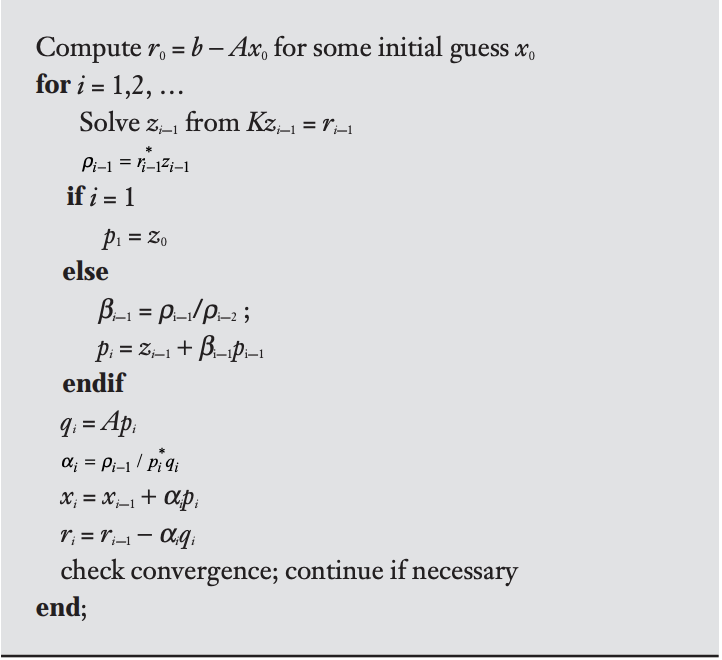
\includegraphics[scale=0.6]{/Users/danny/Documents/UBuffalo/Semester_8_2021/PHY506_CompPhys2/Final_Project/Midsemester_Update/CG_Algorithm.png}
\end{center}
\caption{The conjugate gradients algorithm \cite{Henk2000}.}
\label{CGAlg}
\end{figure}
In more detail, starting with some initial guess $x_0$,  the first residual is calculated using, 
\begin{equation}
r_0 = b - A x_0.
\end{equation}
In each successive CG iteration, the iterates $x_i$ are updated by a multiple $\alpha_i$ of the search direction $p_i$, 
\begin{equation}
x_i = x_{i-1} + \alpha_i p_i,
\end{equation}
and the residual is updated with the equation,
\begin{align}
r_i = r_{i-1} &- \alpha_i q_i \;\; where, \\
q_i &= A p_i.
\end{align}
The constant,
\begin{equation}
\alpha_i = \frac{r_{i-1}^T r_{i-1}}{p_i^T q_i} 
\end{equation}
is chosen to minimize $r_i^T A^{-1} r_i$ over all possible $\alpha_i$.  The search directions $p_i$ are updated using the residuals,
\begin{equation}
p_i = r_i + \beta_{i-1} p_{i-1},
\end{equation}
where,
\begin{equation}
\beta_i = \frac{r_{i}^T r_{i}}{r_{i-1}^T r_{i-1}},
\end{equation}
is chose to ensure $p_i$ and $Ap_{i-1}$ are orthogonal.  Equivalently, this implies any two successive residuals, $r_{i-1}$ and $r_i$, are also orthogonal.  The process of orthogonalizing the search directions and residuals is called \textit{Gram-Schmidt Process} \cite{Keener2000}.  Furthermore, it can be shown that the choice of $\beta_i$ makes the search direction $p_i$ and the residual $r_i$ orthogonal to all previous iterations. 

One main draw of the CG method is that, while the size of the Krylov subspaces can be quite large, the number of vectors that are actually kept in the memory is small.  Additionally the time complexity for CG, given a finite element formulation of a second-order elliptic boundary value problem, is $\mathcal{O}^{3/2}$ in 2D and $\mathcal{O}^{4/3}$ in 3D \cite{Shewchuk1994}. Recalling that the comlexity for Guassian Elimination is $\mathcal{O}^{3}$, this is a considerable improvement in efficiency.

\subsection{Multigrid Methods}

Since their first description in the 60s, multigrid methods have become well known for being the fastest numerical method for solving elliptic boundary value problems.  A good derivation and explanation of multigrid methods is given in \cite{Briggs2000}, but we will provide some of the basic methodologies here. The basic concept behind multigrid is to provide a fine grid solver with a good initial guess obtained from a (or a sequence of) coarse grid solve(s) \cite{Briggs2000}.  Relaxation (or iterative) methods are typically represented by Jacobi or Gauss-Seidel iteration.  To start, consider the simple Two-Grid Correction Scheme ($v^h \leftarrow MG(v^h, f^h)$):
\begin{itemize}
\item Relax $\nu_1$ times on $A^h u^h = f^h$ on $Ω^h$ with initial guess $v_h$.
\item Compute the fine-grid residual $r^h = f^h - A^h v^h$ and restrict it to the coarse grid by $r^{2h} = I^{2h}_h r^h$.
\item Solve $A^{2h}e^{2h} = r^{2h}$ on $Ω^{2h}$.
\item Interpolate the coarse-grid error to the fine grid by $e^h = I^h_{2h} e^{2h}$ and correct the fine-grid approximation by $v^h \leftarrow v^h + e^h$.
\item Relax $\nu_2$ times on $A^h u^h = f^h$ on $\Omega^h$ with initial guess $v^h$.
\end{itemize}
Here, $\Omega^h$ is the finest discretization level and $\Omega^2h$ is the coarse grid, $u^h$ is the solution vector, $v^h$ is the current iterate approximate solution, $r^h$ is the residual, $e^h = u^h - v^h$ is the error and $I^h_{2h}$ is the interpolation operator that takes coarse-grid vectors and produces fine-grid vectors.  In practice $\nu_1$ is usually 1,2 or 3.  In the scheme, relaxation on the fine grid eliminates the oscillatory components of the error, leaving behind only the smooth error.  The smooth error leads to a very good interpolation on the fine grid meaning the correction should be effective. 

As described above, the two-grid correction scheme still leaves room for some improvements.  Primarily, a more direct solution of the residual equation is possible by applying recursion to the coarse-grid correction.  This leads to the more common multigrid scheme, the V-Cycle Scheme ($v^h \leftarrow V^h (v^h, f^h)$):
\begin{itemize}
\item Relax on $A^h u^h = f^h$ $\nu_1$ times with initial guess $v_h$.
\item Compute $f^{2h} = I^{2h}_h r^h$.
	\begin{itemize}
	\item[$\bullet$] Relax on $A^{2h} u^{2h} = f^{2h}$ $\nu_1$ times with initial guess $v^{2h} = 0$.
	\item[$\bullet$] Compute $f^{4h} = I^{4h}_{2h} r^{2h}$.
		\begin{itemize}
		\item[$\bullet$] Relax on $A^{4h} u^{4h} = f^{4h}$ $\nu_1$ times with initial guess $v^{4h} = 0$.
		\item[$\bullet$] Compute $f^{8h} = I^{8h}_{4h} r^{4h}$.
			\begin{itemize}
				\item[$\vdots$]
				\item Solve $A^{Lh} u^{Lh} = f^{Lh}$.
				\item[$\vdots$]
			\end{itemize}
		\item[$\bullet$] Correct $v^{4h} \leftarrow v^{4h} + I^{4h}_{8h} v^{8h}$.
		\item[$\bullet$] Relax on $A^{4h} u^{4h} = f^{4h}$ $\nu_2$ times with initial guess $v^{4h}$.
		\end{itemize}
	\item[$\bullet$] Correct $v^{2h} \leftarrow v^{2h} + I^{2h}_{4h} v^{4h}$.
	\item[$\bullet$] Relax on $A^{2h} u^{2h} = f^{2h}$ $\nu_2$ times with initial guess $v^{2h}$.
	\end{itemize}
\item Correct $v^{h} \leftarrow v^{h} + I^{h}_{2h} v^{2h}$.
\item Relax on $A^{h} u^{h} = f^{h}$ $\nu_2$ times with initial guess $v^{h}$.
\end{itemize}

The V-Cycle is just one of many different multigrid schemes.

\subsection{Helmholtz Equation}

\subsubsection{Good Cop vs. Bad Cop}


Solving the general Helmholtz equation, 
\begin{equation}
-\Delta u + k^2 u = f,
\end{equation} 
with numerical methods, and particularly multigrid methods, is an open problem \cite{Ernst2012}.  We will briefly touch upon why this is in this section before moving forward with the formulation used in this project.  For simplicity, we consider only the cases where $k^2=+1$ and $k^2=-1$, respectively referred to as "Good Cop" and "Bad Cop" Helmholtz equations.  First, we introduce the concepts of \textit{positive definite} and \textit{negative definite} matrices.

\begin{definition}
A $n \times n$ Hermitian matrix, $A$, is said to be \textbf{positive definite} if the scalar $z^* A z$ is \textit{positive} for all real, non-zero column vectors $z$ of size $n$.  Here, $z^*$ denotes the conjugate transpose of the vector $z$.  If however $z^* A z$ is \textit{negative}, then $A$ is called a \textbf{negative definite} matrix.  Lastly, if $z^* A z$ can be either \textit{positive} or \textit{zero}, then it is called \textbf{positive semi-definite}, and, similarly, if $z^* A z$ can be either \textit{negative} or \textit{zero}, it is called \textbf{negative semi-definite} \cite{Keener2000}.
\label{PosDef}
\end{definition}

It is worth noting that the existence of positive, negative or zero eigenvalues of a matrix can also be used to define what type of matrix $A$ is.  Since we strive to convert our initial equation formulation $-\Delta u + k^2 u = f$, also called the \textit{strong form}, to a linear system $Au=f$, we can extend \eqref{PosDef} to the strong form of our equations where $A=-\Delta + k^2$.  Furthermore, in numerical methods, a positive definite operators are highly desirably as they can be easily inverted and contain other useful properties.  

The negative Laplacian operator, $-\Delta$, is well known for being a positive definite operator.  Therefore, the positive definiteness of the Helmholtz equation is dependent on the $k^2$ term.  If $k^2 \geq 0$, i.e. the "Good Cop" form, then the equation remains positive definite and is solvable with common methods.  However, if $k^2 \leq 0$, i.e. the "Bad Cop" form, then the equation becomes indefinite and solution becomes much trickier.  As stated at the beginning of this section, solving the indefinite form of the Helmholtz equation is still an open research topic of interest.


\subsubsection{Variational Formulation}
For the reasons given in the previous section, we consider only the case where $k^2=+1$, or the "Good Cop" Helmholtz equation \cite{Farrell2018},
\begin{figure}[!ht]
\begin{center}
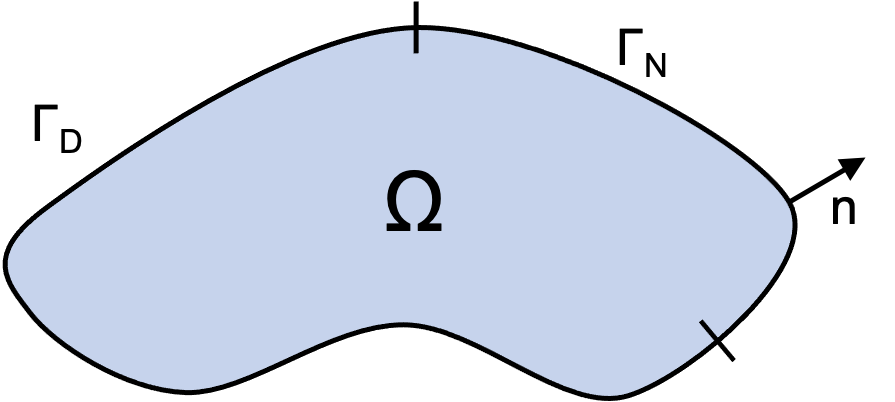
\includegraphics[scale=0.6]{/Users/danny/Documents/UBuffalo/Semester_8_2021/PHY506_CompPhys2/Final_Project/Midsemester_Update/Domain.png}
\end{center}
\caption{General domain for solving}
\label{Domain}
\end{figure}
\begin{align}
-\Delta u + u &= f \;\; in \;\; \Omega, \\
u &= u_0 \;\; on \;\; \Gamma_D \subset \partial \Omega, \\
\nabla u\cdot n &= g \;\; on \;\; \Gamma_N \subset \partial \Omega.
\label{pde}
\end{align}
To discretize this equation, we use the finite elements method.  The first step in discretization is to derive a weak (or variational) formulation.  The process used to derive the weak form for the "Good Cop" Helmholtz equation in this project can be found in \cite{AutomatedFEM2011} and \cite{Fenics2017}.  We start by multiplying by a test function $v$ and integrating over the domain to obtain,
\begin{equation}
-\int_{\Omega} (\Delta u) \, v \, dx + \int_{\Omega} u \, v \, dx = \int_{\Omega} f \, v \, dx.
\end{equation}
It is common when deriving weak formulations to try and reduce the order of the derivatives of $u$ and $v$ as much as possible.  In the case of the Helmholtz equation, the laplacian term can be reduce to two first order gradients of $u$ and $v$ using integration by parts.  The integration by parts formula reads,
\begin{align}
-\int_\Omega (\Delta u) \, v \, dx &= \int_\Omega \nabla u \cdot \nabla v - \int_{\Gamma} \frac{\partial u}{\partial n} \, v \, ds, \\
 &= \int_\Omega \nabla u \cdot \nabla v - \int_{\Gamma} \nabla u \cdot v \, ds,
\end{align}
where $\frac{\partial u}{\partial n} = \nabla u \cdot n$ is the derivative of $u$ in the normal direction $n$ on the boundary.  We note that Gauss' Theorem is used to replace the volume integral with the surface integral.  Using this formula on the Helmholtz equation gives, 
\begin{equation}
\int_{\Omega} \nabla u \cdot \nabla v \, dx - \int_{\Gamma_N} v \, (\nabla u \cdot n) \, ds + \int_{\Omega} u \, v \, dx = \int_{\Omega} f \, v \, dx.
\end{equation}

Another common rule when deriving weak formulations is that the test function $v$ vanishes on the parts of the boundary where the solution $u$ is known.  This requirement is explained in detail in \cite{Langtangen2019}.  Presently, this means $v=0$ on the entire boundary $\partial \Omega$ simplifying the weak form to,
\begin{equation}
\int_{\Omega} \nabla u \cdot \nabla v \, dx + \int_{\Omega} u \, v \, dx = \int_{\Omega} f \, v \, dx.
\end{equation}
We require that this formulation holds true for all test functions $v$ in some \textit{test space} $\hat{V}$.  From this requirement, we can then determines a unique solution $u$ which lies in some function space $V$, also called a \textit{trial space}.  For this problem, the test and trial spaces, $V$ and $\hat{V}$, are defined as,
\begin{align}
V = \lbrace v \in H^1 (\Omega) : v=u_0 \; on \; \partial \Omega \rbrace, \\
\hat{V} = \lbrace v \in H^1 (\Omega) : v=0 \; on \; \partial \Omega \rbrace,
\end{align}
where $H^1 (\Omega)$ is the well-known Sobolev space containing the functions $v$ such that $v^2$ and $|\nabla v|^2$ have finite integrals over $\Omega$.  Therefore, the continuous solution of the Helmholtz PDE must lie in a function space where the derivatives are also continuous, however the Sobolev space $H^1 (\Omega)$ allows functions with discontinuous derivatives.  This weaker continuity condition of $u$ in the weak formulation allows the use of piecewise polynomial function spaces, or simply put function spaces constructed by stitching together polynomial functions on simple domains such as intervals (1D), triangles (2D) or tetrahedrons (3D). 

The next step is to replace the infinite-dimensional function spaces $V$ and $\hat{V}$ with discrete (finite-dimensional) trial and test spaces $V_h \subset V$ and $\hat{V}_h \subset \hat{V}$.  We define the discrete form of $u$, $u_h \in V_h \subset V$ and plug it back into the variational formulation which gives the discretretized weak form,
\begin{equation}
\int_{\Omega} \nabla u_h \cdot \nabla v \, dx + \int_{\Omega} u_h \, v \, dx = \int_{\Omega} f \, v \, dx \;\; \forall v \in \hat{V_h} \subset \hat{V}.
\end{equation}
This discretized weak form along with suitable definitions of the discrete trial and test spaces $V$ and $\hat{V}$ define the approximate numerical solution for the "Good Cop" Helmholtz equation.  We assume that we have a basis $\lbrace \phi_j \rbrace^N_{j=1}$ for $V_h$ and a basis $\lbrace \hat{\phi}_i\rbrace^N_{i=1}$ for $\hat{V}_h$, where N is the dimension of the space $V_h$.  We can then make an ansatz for $u_h$ in terms of the basis functions of the trail space,
\begin{equation}
u_h (x) = \sum^N_{j=1} U_j \phi_j(x),
\end{equation}
where $U \in \mathbb{R}^N$ is the vector of defrees of freedom to be computed \cite{AutomatedFEM2011}.  Plugging the bases into the variational form gives,
\begin{equation}
\sum^N_{j=1} U_j \int_{\Omega} \nabla \phi_j \cdot \nabla \phi_i \, dx + \sum^N_{j=1} U_j \int_{\Omega} \phi_j \, \phi_i \, dx = \int_{\Omega} f \, \phi_i \, dx \;\;\; i = 1,2,...,N.
\end{equation}

Therefore,a finite element solution $u_h (x) = \sum^N_{j=1} U_j \phi_j(x),$ can be computed for this system by solving the linear system,
\begin{equation}
A U = b
\end{equation}
where,
\begin{align}
A_{ij} &= \int_{\Omega} \nabla \phi_j \cdot \nabla \phi_i \, dx + \int_{\Omega} \phi_j \, \phi_i \, dx \\
b_i &= \int_{\Omega} f \, \phi_i \, dx.
\end{align}

\subsubsection{Method of Manufactured Solutions}

Thus far, we have used a generalized form of the "Good Cop" Helmholtz equation, including some function $f$ and domain $\Omega$, to derive the necessary formulations needed for our code.  For the implementation, however, we require some specific choices for $f$, $\Omega$ and $u_0$.  Furthermore, it is wise to first choose an exact solution for $u$ and   derive $f$, $\Omega$ and $u_0$ based on the exact solution.  This process is referred to as the \textit{Method of Manufactured Solutions}.  Therefore, we choose our exact solution to be,
\begin{equation}
u_e(x,y) = 1 + x^2 + 2 y^2.
\end{equation}
Inserting $u_e$ into equation \eqref{pde} we find that $u_e$ is a solution if,
\begin{align}
f(x,y) = -5 + x^2 + 2 y^2, \\
u_0(x,y) = 1 + x^2 + 2 y^2.
\end{align}
We also choose the domain to be,
\begin{equation}
\Omega = [0,1] \times [0,1].
\end{equation}
Finally, plugging $f$ into the discretized variational form gives,
\begin{equation}
\sum^N_{j=1} U_j \int_{\Omega} \nabla \phi_j \cdot \nabla \phi_i \, dx + \sum^N_{j=1} U_j \int_{\Omega} \phi_j \, \phi_i \, dx = \int_{\Omega} (-5 + x^2 + 2 y^2) \, \phi_i \, dx \;\;\; i = 1,2,...,N.
\end{equation}



\subsubsection{PETSc Formulation}

In PETSc, the \textit{primal problem} is set by the functions PetscDSSetExactSolution, PetscDSSetResidual and PetscDSSetJacobian.  Each function requires a specific equation form as the inputs.  The residual function is requires the form,
\begin{equation}
\int_\Omega \phi_i f_0(u, u_t, \nabla u, x, t) + \nabla\phi_i \cdot {\vec f}_1(u, u_t, \nabla u, x, t),
\end{equation}
and the jacobian function takes the form,
\begin{equation}
\begin{split}
\int_\Omega &\phi_i g_0(u, u_t, \nabla u, x, t) \phi_j + \\
&\phi_i {\vec g}_1(u, u_t, \nabla u, x, t) \nabla \phi_j + \\
&\nabla\phi_i \cdot {\vec g}_2(u, u_t, \nabla u, x, t) \phi_j + \\
&\nabla\phi_i \cdot {\overleftrightarrow g}_3(u, u_t, \nabla u, x, t) \cdot \nabla \phi_k.
\end{split}
\end{equation}
Therefore, in the multigrid code we use the function inputs,
\begin{align}
f_0 &= u - (-5 + x^2 + 2 y^2), \\
f_1 &= \nabla u, \\
g_0 &= 1.0, \\
g_1 &= 0.0, \\
g_2 &= 0.0,\; and \\
g_3 &= 1.0.
\end{align}


\section{Implementation}



\subsection{GPU Code}



\printbibliography 

\end{document}



